\documentclass[tikz]{standalone}
\usepackage{amsmath}
\definecolor{bgdark}{HTML}{171D2B}
\definecolor{aksen}{HTML}{F7B538}
\begin{document}
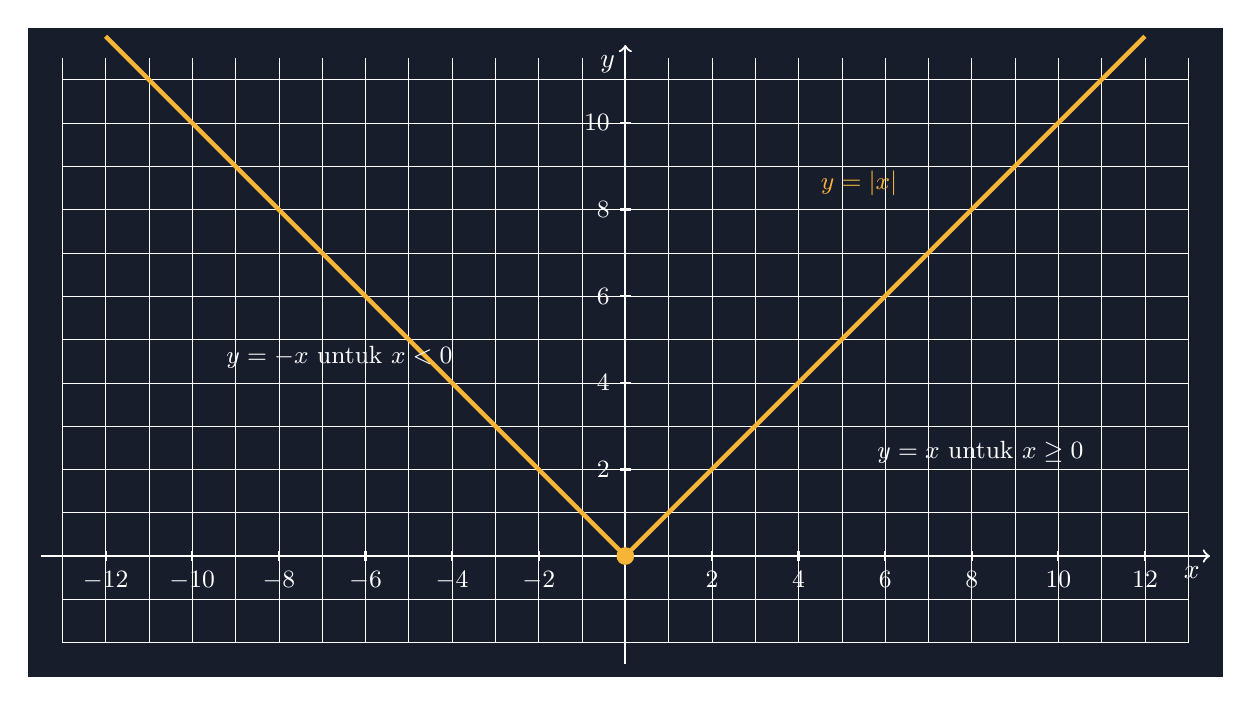
\begin{tikzpicture}[x=0.55cm,y=0.55cm]
\fill[bgdark] (-13.8,-2.8) rectangle (13.8,12.2);
\begin{scope}
\draw[white!25,very thin] (-13,-2) grid[step=1] (13,11.5);
\draw[->,white!70,thick] (-13.5,0) -- (13.5,0) node[below left,white!80] {$x$};
\draw[->,white!70,thick] (0,-2.5) -- (0,11.8) node[below left,white!80] {$y$};
\foreach \i in {-12,-10,-8,-6,-4,-2,2,4,6,8,10,12}{
  \draw[white!70,thick] (\i,0.12) -- (\i,-0.12) node[below,white!80,font=\small] {$\i$};}
\foreach \j in {2,4,6,8,10}{
  \draw[white!70,thick] (0.12,\j) -- (-0.12,\j) node[left,white!80,font=\small] {$\j$};}
\draw[aksen,line width=1.6pt] (-12,12) -- (0,0) -- (12,12);
\fill[aksen] (0,0) circle (3.2pt);
\node[aksen,font=\small\bfseries] at (5.4,8.6) {$y=|x|$};
\node[white!80,font=\small] at (8.2,2.4) {$y=x$ untuk $x\ge 0$};
\node[white!80,font=\small] at (-6.6,4.6) {$y=-x$ untuk $x<0$};
\end{scope}
\end{tikzpicture}
\end{document}
